

%%%%%%%%%%%%%%%%%%%%%%%%%%%%%%%%%%%%%%%%%%%%%%%%%%%%%%%%%%%%%%%%%%%%%%
%%%%%%%%%%%%%%%% Convolutional Networks for Semantic Segmentation
%%%%%%%%%%%%%%%%%%%%%%%%%%%%%%%%%%%%%%%%%%%%%%%%%%%%%%%%%%%%%%%%%%%%%%

\section{Convolutional Networks for Semantic Segmentation}
\label{sec:cnn4seg}

\subsection{Convolutional Neural Networks}
\label{subsec:cnn}

%%%%%%%% CNN in one sentence

The main components of a typical convolutional neural network (CNN) are several layers of convolutions and sub-sampling, followed by a few fully-connected layers.


%%%%%%%% FIGURE LeNet
\begin{figure}[t]
\centering
   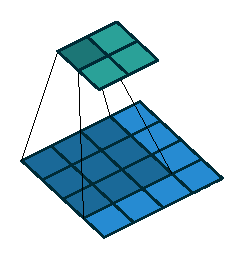
\includegraphics[width=\linewidth]{img/no_padding_no_strides_00.pdf}
\caption{
A basic convolution operation.
A 3x3 convolutional filter convolves with a 3x3 window sliding over the image (bottom).
The output of convolutions at each sliding position form a feature map (top).
This figure was drawn by Dumoulin and Visin \cite{dumoulin2016guide}
}
\label{fig:conv}
\end{figure}

%%%%%%%% LeNet

An example CNN model, LeNet-5 (1998) \cite{lecun1998gradient}, is shown in Figure \ref{fig:lenet}.
The first convolutional layer of LeNet contains 6 convolutional kernels of size 5x5 and each convolutional kernels convolve with small windows sliding over the images and produce a feature map of size 28x28.
Each output in the produced feature map is corresponding to a small sub-region of the visual field (the image), called a \textit{receptive field}.
A following max pooling layer subsamples the feature maps by a factor of two by extracting the maximum values for every two adjacent pixels literally and vertically.
The result feature map S2 has a shape of 14 by 14 and a receptive field of 6 by 6.
Another sequence of convolutional and pooling layers generate feature maps of size 5x5 with receptive field 16x16.
Neurons in the last three layers of LeNet are fully connected to the layer before and the layer after if exists, creating the final prediction for 10 classes.

%%%%%%%% Feature Hierarchy
Features produced by CNN models have a rich hierarchy varying from local to global, from simple to complex.
The bottom layers in the convolutional layer stack have smaller receptive fields while the top layers have larger receptive fields.
A small receptive field means that the filter have access to information only in a local sub-region of the image while a large receptive field can convey more global information.

The various pattern responses from local to global, from simple to complex for stacked convolutional layers is a reflect of emulating animals visual cortex.
In cat's visual cortex \cite{hubel1962receptive}, two basic cell types of visual cortex have been identified:
Simple cells respond maximally to specific edge-like patterns within their receptive field.
Complex cells have larger receptive fields and are locally invariant to the exact position of the pattern.
The shallower convolutional layers play a similar functionlity as simple cells while the deeper layers maps are similar to complex cells.

%%%%%%%% FIGURE LeNet
\begin{figure}[t]
\centering
   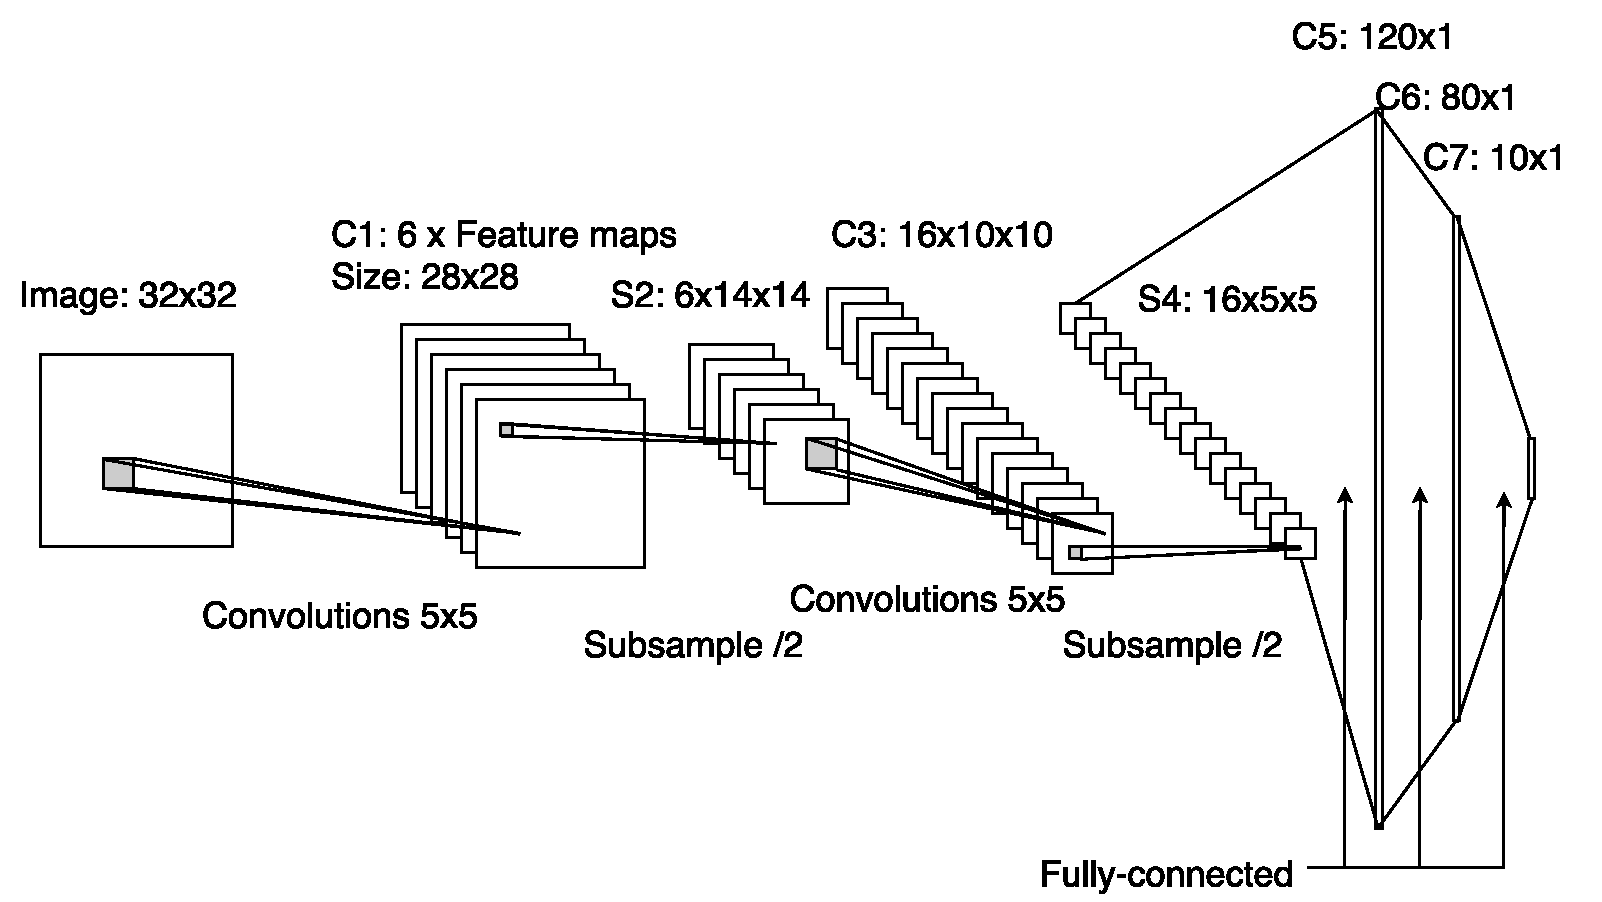
\includegraphics[width=\linewidth]{img/lenet}
\caption{An example convolutional neural network, LeNet-5 \cite{lecun1998gradient}}
\label{fig:lenet}
\end{figure}

%%%%%%%% Design of CNN

The main benefit of CNN compared to a standard multilayer neural network (multilayer perceptron) is that
1. take advantage of the 2D structure of an input image
2. it is easier to optimize because of spatial weights sharing and local connectivy pattern of convolutional layers.
Convolutional neurons and maximum pooling, translation invariance as well as scaling invariance and distortion invariance to some extent are achievable for convolutional neural networks. \cite{lecun1998gradient}
Different from the traditional handcrafted features, learnable convolutional features normally generalize well and can achieve better performance for dataset with a complex input distribution. \cite{krizhevsky2012imagenet}
By increasing the number of convolution layers and number of filters in each layer, one can create CNN models with high capacity, meaning a large space of representable functions.
This can be beneficial for datasets of immense complexity, for example, ILSVRC \cite{russakovsky2015imagenet}, Microsoft COCO \cite{lin2014microsoft}, as long as there are sufficient training samples with an appropriate optimization strategy.


\subsection{Semantic image segmentation}
\label{subsec:segmentation}

%%%%%%%% Segmentation in one sentence

Semantic image segmentation is to segment images into semantically meaningful partitions, a.k.a.,\textit{segments}.
It can be operated as classifying pixels into the corresponding pre-defined categories.

%%%%%%%% Difficulty in adapting CNN

CNN models on object classification tasks can be adapted to perform semantic image segmentation tasks. \cite{long2015fully}
One of the primary difficulties of applying CNN model to segmentation tasks is how to combine global information and local information to solve semantics and locations altogether.
In contrast to object classification tasks, which normally only need global information to resolve semantics, segmentation tasks also require local information to resolve locations.

%%%%%%%% An example segmentation framework: FCN

Long et al. \cite{long2015fully} proposed a so-called skip architecture in Fully convovolutional networks (FCN) to aggregate information from the local low-level features in the hierarchy with global information from the high-level features.
As we discussed in the previous session, convolutional layers can extract hierarchical features, which from low-level to high-level encode information from local to global.
The low-level features are fine, presenting appearances and the high-level features are coarse, revealing semantics.
By combining them together, it becomes possible to create accurate and detailed segmentation.
% in an end-to-end, pixel-by-pixel fully convolutional neural networks for semantic segmentation.%%%%%%%% FIGURE LeNet


\begin{figure}[t]
\centering
   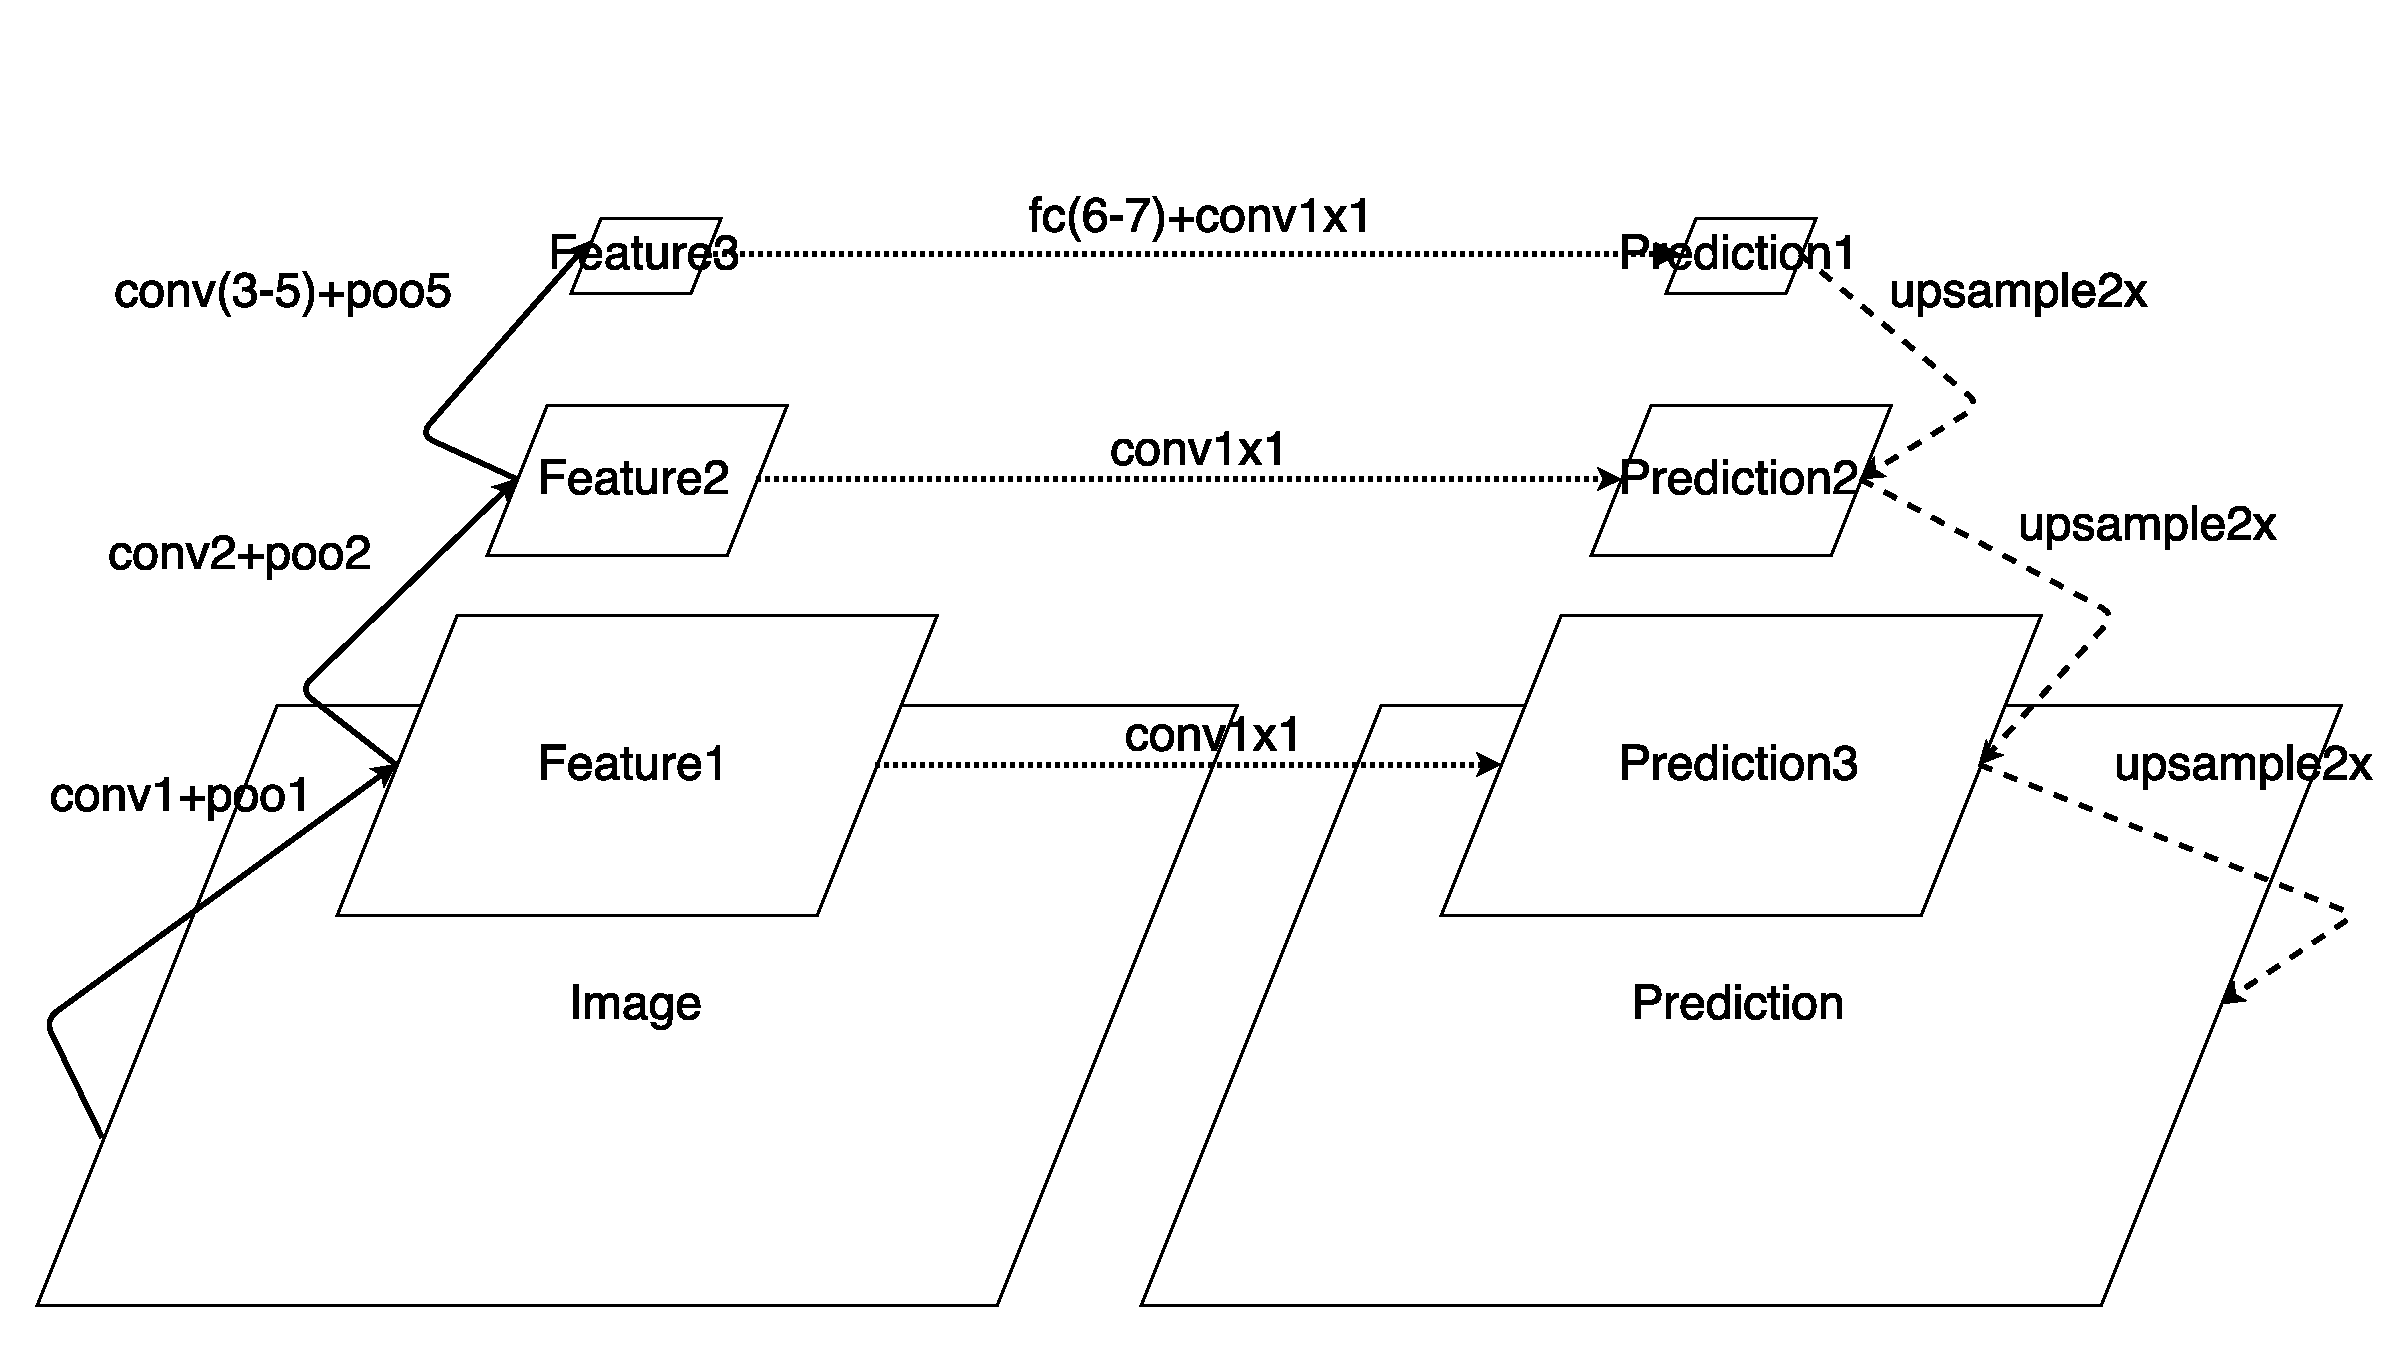
\includegraphics[width=\linewidth]{img/fcn}
\caption{Fully convolutional network (FCN) by Long et al. (2015)  \cite{long2015fully}.}
\label{fig:fcn}
\end{figure}

%%%%%%%% Transferring convolutional neural nets

Convolutional layers in FCN for feature extractions (solid arrows in Figure \ref{fig:fcn}) can be transferred from ImageNet models.
